% !TEX program = xelatex
% akizumi-tikz: tikz=full libraries, plots, and every semantic style
\documentclass[tikz=full, plots]{akizumi-note}
\begin{document}
\section{Arrays and flowcharts}
\begin{tikzpicture}[x=0.9cm]
  \foreach \v [count=\i from 0] in {7,2,9,4,1} {
    \node[akizumi/cell] (c\i) at (\i,0) {\v};
    \node[akizumi/index, below=1pt] at (c\i.south) {\i};
  }
  \node[akizumi/hlcell] at (2,0) {9};
  \node[akizumi/hlcell2] at (4,0) {1};
  \draw[akizumi/arrow] (c2.north) to[bend left=40] (c4.north);
  \draw[decorate, decoration={brace, amplitude=4pt, mirror}, draw=mute]
    (-0.5,-1) -- node[akizumi/note, below=4pt] {sorted} (1.5,-1);
\end{tikzpicture}

\begin{tikzpicture}[node distance=0.6cm and 1.2cm]
  \node[akizumi/start] (s) {start};
  \node[akizumi/io, below=of s] (in) {read $n$};
  \node[akizumi/decision, below=of in] (d) {$n > 0$?};
  \node[akizumi/process, right=of d] (p) {$n \gets n - 1$};
  \node[akizumi/start, below=of d] (e) {end};
  \draw[akizumi/arrow] (s) -- (in);
  \draw[akizumi/arrow] (in) -- (d);
  \draw[akizumi/arrow] (d) -- node[akizumi/note, above] {yes} (p);
  \draw[akizumi/arrow] (p) |- (in);
  \draw[akizumi/arrow] (d) -- node[akizumi/note, right] {no} (e);
  \begin{scope}[on background layer]
    \node[akizumi/group, fit=(d) (p)] {};
  \end{scope}
\end{tikzpicture}

\section{Automata and game trees}
\begin{tikzpicture}[akizumi/automaton]
  \node[state, initial] (q0) {$q_0$};
  \node[state, accepting, right=of q0] (q1) {$q_1$};
  \path[->] (q0) edge["$a$"] (q1)
            (q1) edge[loop above] node {$b$} ()
            (q1) edge[bend left, "$a$"] (q0);
\end{tikzpicture}
\qquad
\begin{tikzpicture}[x=1.4cm, y=1cm]
  \node[akizumi/game/chance, label=above:{N}] (n) at (-1.2,0) {};
  \node[akizumi/game/decision, label=above:{Amy}] (a) at (0,0) {};
  \node[akizumi/game/decision] (b1) at (1.5,1) {};
  \node[akizumi/game/decision] (b2) at (1.5,-1) {};
  \draw[akizumi/game/branch] (n) -- (a);
  \draw[akizumi/game/branch] (a) -- node[akizumi/game/action, above left] {$H$} (b1);
  \draw[akizumi/game/branch] (a) -- node[akizumi/game/action, below left] {$F$} (b2);
  \foreach \b/\y/\p in {b1/1.5/{(1,-1)}, b1/0.5/{(-1,1)}, b2/-0.5/{(-1,1)}, b2/-1.5/{(1,-1)}} {
    \node[akizumi/game/terminal, label={[akizumi/game/payoff]right:$\p$}] (t) at (3,\y) {};
    \draw[akizumi/game/branch] (\b) -- (t);
  }
  \draw[akizumi/game/infoset] (b1) -- node[akizumi/note, right] {Bart} (b2);
\end{tikzpicture}

\section{Physics and 3D}
\begin{tikzpicture}
  \draw[akizumi/wire] (0,0) rectangle (2.4,1.6);
  \pic at (0,1.6) {akizumi/current in};
  \pic at (2.4,1.6) {akizumi/current out};
  \pic[accent] at (0,0) {akizumi/current out};
  \pic[warn] at (2.4,0) {akizumi/current in};
  \coordinate (O) at (1.2,0.8); \coordinate (X) at (2.4,0.8); \coordinate (Y) at (1.2,1.6);
  \pic[draw=mute, "$\theta$", angle radius=0.45cm] {angle=X--O--Y};
\end{tikzpicture}
\qquad
\begin{tikzpicture}[x={(0.8cm,-0.3cm)}, y={(0.9cm,0.2cm)}, z={(0cm,0.9cm)}]
  \begin{scope}[canvas is xy plane at z=0]
    \draw[pattern=north east lines, pattern color=mute] (0,0) rectangle (1.5,1.5);
  \end{scope}
  \draw[akizumi/arrow] (0,0,0) -- (2,0,0) node[akizumi/note, right] {$x$};
  \draw[akizumi/arrow] (0,0,0) -- (0,2,0) node[akizumi/note, right] {$y$};
  \draw[akizumi/arrow] (0,0,0) -- (0,0,1.8) node[akizumi/note, above] {$z$};
\end{tikzpicture}
Marked\tikzmark{m}.

\section{Plots}
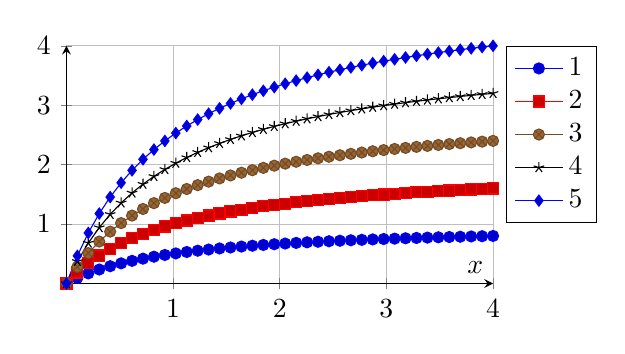
\begin{tikzpicture}
  \begin{axis}[width=7cm, height=4.6cm, axis lines=middle, grid=major, xmin=0, xmax=4,
      legend pos=outer north east, xlabel={$x$}]
    \foreach \k in {1,...,5} { \addplot+[domain=0:4, samples=40] {\k*x/(1+x)}; }
    \legend{$1$,$2$,$3$,$4$,$5$}
  \end{axis}
\end{tikzpicture}
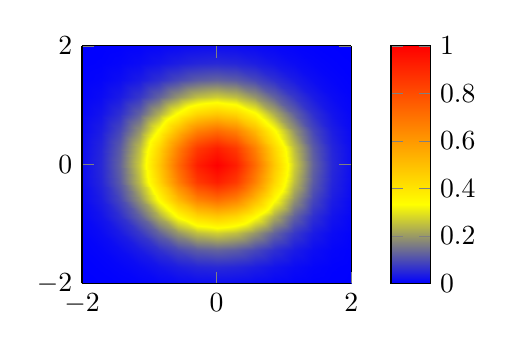
\begin{tikzpicture}
  \begin{axis}[width=5cm, height=4.6cm, view={0}{90}, colorbar]
    \addplot3[surf, shader=interp, domain=-2:2, samples=15] {exp(-x^2-y^2)};
  \end{axis}
\end{tikzpicture}
\end{document}
